\section{Paradigms for parametric search}
\label{sec:prelims}

In this section we discuss features of parametric search,
and lay the foundation for the optimal algorithms
that we give in subsequent sections.
We first review straightforward feasibility tests
to test the feasibility of a search value in a tree.
We then review how to represent all possible search values
of a path within a ``sorted matrix''. 
We next present a general approach for search that
uses values from a collection of sorted matrices.
Finally, we describe straightforward approaches
for the path and the tree that are as good as any
algorithms in \cite{M,C2}.

We first describe straightforward feasibility tests for cutting edges in a tree so as to maximize the minimum weight of any resulting component (max-min problem).
The feasibility test takes a test value $\lambda$, and determines if at least $k$ cuts can be placed in the tree
such that no component has weight less than $\lambda$. 
We take $\lambda^*$ to be the largest value that passes the test.

A straightforward test for the max-min problem in a tree is given in \cite{M},
and the feasibility test for the min-max problem is similar \cite{KM}. 
We focus first on max-min, using an algorithm {\it FTEST0}, which starts 
by rooting the tree at a vertex of degree 1
and initializing the number of cuts, $numcut$, to $0$.
It next calls {\it explore}$({\it root})$ to explore the tree starting at the root.
When the exploration is complete,
if $numcut > k$,
then $\lambda$ is a lower bound on $\lambda^*$,
and otherwise $\lambda$ is an upper bound on $\lambda^*$.
The procedure {\it explore} is:

\bigskip
\sspace
\noindent
{\bf proc} {\it explore} $({\bf vertex} ~v)$\vspace{.05in}\\
$\T $ {\it accum\_wgt}$(v)$ $\ASG$ weight of $v$\vspace{.05in}\\
$\T $ $\FO$ each child $w$ of $v$ $\DO$ ${\it explore(w)}$ $\EF$\vspace{.05in}\\
$\T $ Adjust {\it accum\_wgt}$(v)$ and $numcut$.
 
\dspace
\bigskip
\noindent
For the max-min problem, we adjust {\it accum\_wgt}$(v)$ and $numcut$ by:

\bigskip
\sspace
\noindent
$\T $ $\FO$ each child $w$ of $v$ $\DO$ Add ${\it accum\_wgt}(w)$ to ${\it accum\_wgt}(v)$. $\EF$\vspace{.05in}\\
$\T $ $\IF$ {\it accum\_wgt}$(v) \geq \lambda$\vspace{.05in}\\ 
$\T $ $\TN$ $numcut \ASG numcut + 1$\vspace{.05in}\\
$\T $ $\T $ {\it accum\_wgt}$(v) \ASG 0$\vspace{.05in}\\
$\T $ $\EI$
 
\dspace
\bigskip


In all but one case, we cut an edge in the tree whenever we increment $numcut$ by 1. 
For the max-min problem, we generally cut the edge from the current vertex $v$ to its parent except for 
the last increment of $numcut$ in {\it FTEST0}.
This is because either $v$ will be the root and thus does not have a parent,
or the fragment of the tree above $v$ will have total weight less than $\lambda$.
By not adjusting $numcut$ to reflect the actual number of cuts in this case,
we are able to state the threshold test for both versions of {\it FTEST0}
in precisely the same form. 
The feasibility test takes constant time per vertex, and thus uses $O(n)$ time.

In a parametric search problem,
the search can be restricted to considering values from a finite set of values.
The desired value is the largest (in the case of a max-min problem)
or the smallest (in the case of a min-max problem)
that passes the feasibility test.
Let each value in the finite set be called a {\it candidate value}.
We next discuss a data structure that contains all candidate
values for problems on just a path.
This structure is based on ideas in \cite{FJ1} and \cite{FJ2}.
Let a matrix be called a {\it sorted matrix}
if for every row the values are in nondecreasing order,
and for every column the values are in nonincreasing order.
(Note that for notational convenience,
this definition varies slightly from the definition in \cite{FJ1}.)
Let the vertices on the path $P$ be indexed from 1 to $n$.

The set of values that we need to search is the set of sums of weights of vertices from $i$ to $j$, for all pairs $i\leq j$. 
We succinctly maintain this set of values, plus others, in a data structure, the \emph{succinct description}. 
For $i=0,1, \cdots ,n$, let $A_i$ be the sum of the weights of vertices 1 to $i$.
Note that for any pair $i,j$ with $i \leq j$, the sum of the weights from vertex $i$ to $j$ is $A_j - A_{i-1}$.
Let $X_1$ be the sequence of sums $A_1, A_2, \cdots ,A_n$, and let $X_2$ be the sequence of sums $A_0, A_1, \cdots ,A_{n-1}$.
Then sorted matrix $M(P)$ is the $n \times n$ Cartesian matrix $X_1-X_2$, where the $ij$-th entry is $A_j-A_{i-1}$.
In determining the above, we can use proper subtraction, in which, $a-b$ gives $\max \{a-b,0\}$.
Clearly, the values in any row of $M(P)$ are in nondecreasing order, and the values in any column of $M(P)$ are in nonincreasing order. 
Representing $M(P)$ explicitly would require $\Theta(n^2)$ time and space. 
Thus, our data structure succinctly represents $M(P)$ (and hence, $P$) in $O(n)$ space by the two vectors $X_1$ and $X_2$. 

In general, our algorithm also needs to inspect specific subpaths of $P$. 
However, repeatedly copying subvectors of $X_1$ and $X_2$ can take more than linear time in total. 
On the other hand, for a subpath $Q$ of $P$, the corresponding matrix $M(Q)$ is a submatrix of $M(P)$, which we can recover from the succinct representation of $P$. 
Thus, our algorithm succinctly represents $M(Q)$ by the start and end indices of $M(Q)$ within $M(P)$. 
In this way, we can generate the values of $M(Q)$ from the vectors $X_1$ and $X_2$ of $M(P)$, as well as the location of the submatrix as given by the succinct representation of $Q$. 
Therefore, our algorithm avoids needlessly recopying vectors and instead generates in $O(n)$ total time the succinct representations of all subpaths that it may inspect.

\begin{figure}[thb]
\begin{center}
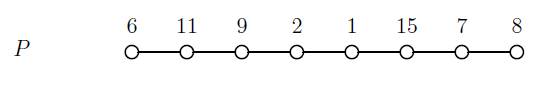
\includegraphics{fig2p1a}
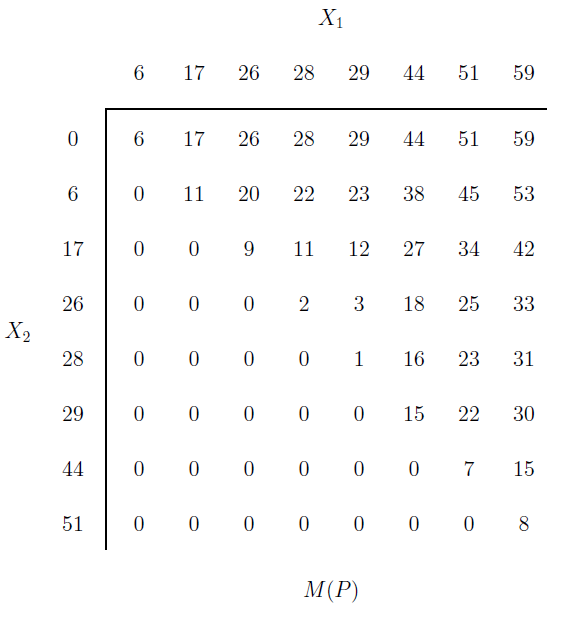
\includegraphics{fig2p1b}
\end{center}
\caption{\small Path $P$, vectors $X_1$ and $X_2$, and explicit illustration of matrix $M(P)$
\label{fig1}}
\end{figure}

As an example, we show a vertex-weighted path $P$ in Fig.~\ref{fig1},
and its associated matrix $M(P)$.
We list the sequence $X_1$ horizontally above $M(P)$,
and the sequence $X_2$ vertically to the left of $M(P)$,
in such a way that the $ij$-th element of $M(P)$
is beneath the $j$-th element of $X_1$
and to the right of the $i$-th element of $X_2$.

We next describe the general form {\it PARAM\_SEARCH} of all of our searching algorithms.
It is related to, and uses some of the ideas in, algorithms found in \cite{C2}, \cite{FJ1}, \cite{FJ2}, and \cite{M}.
By specifying the specific subroutines {\it INIT\_MAT}, {\it TEST\_VAL}, {\it UPDATE\_MAT},  we will be able to give four versions of {\it PARAM\_SEARCH}, namely {\it PATH0}, {\it TREE0}, {\it PATH1}, and {\it TREE1}.
In all four versions, {\it PARAM\_SEARCH} takes as its arguments an integer $k$ and either a vertex-weighted path or a tree.
It initializes searching bounds $\lambda_1$ and $\lambda_2$, where $\lambda_1 < \lambda_2$. 
The algorithm progressively narrows these bounds until they satisfy the following conditions by the end of the algorithm.
For a max-min problem, $\lambda_1$ is the largest value that is feasible,
and $\lambda_2$ is the smallest value that is not feasible.
(For a min-max problem, $\lambda_1$ is the largest value that is not feasible,
and $\lambda_2$ is the smallest value that is feasible.)

{\it PARAM\_SEARCH} will use {\it INIT\_MAT} to initialize $\cal M$,
a collection of succinctly represented square sorted matrices,
the union of whose values is the set of values that we consider.
{\it PARAM\_SEARCH} then performs a series of iterations.
On each iteration, it will use {\it TEST\_VAL} to identify and test a
small number of values $\lambda$
drawn from matrices in $\cal M$.
Each value $\lambda$ will be either the largest or the smallest element
in some matrix in $\cal M$.
As a result of the feasibility tests,
{\it UPDATE\_MAT} updates $\mathcal{M}$ by deleting 
certain matrices from $\cal M$,
dividing certain matrices into 4 submatrices,
and inserting certain matrices into $\cal M$.
Note that in initializing $\lambda_2$ to $\infty$,
we take $\infty$ to be any value greater than the total weight
of all vertices in the path or the tree.

\bigskip
\sspace
\noindent
{\bf Algorithm} {\it PARAM\_SEARCH}\vspace{.05in}\\
$\T $ $\lambda_1 \ASG 0$\\
$\T $ $\lambda_2 \ASG \infty$\vspace{.05in}\\
$\T $ {\it INIT\_MAT}\vspace{.05in}\\
$\T $ $\WH$ $\cal M$ is not empty $\DO$\vspace{.05in}\\
$\T \T $ {\it TEST\_VAL}\vspace{.05in}\\
$\T \T $ {\it UPDATE\_MAT}\vspace{.05in}\\
$\T $ $\EW$\\
$\T $ Output $\lambda_1$ and $\lambda_2$.\\
$\T $ /* For max-min, $\lambda^*$ will be the final $\lambda_1$ and for min-max, $\lambda^*$ will be the final $\lambda_2$. */
 
\dspace
\bigskip

In the remainder of this section we
describe simple algorithms {\it PATH0} and {\it TREE0}
for partitioning a path and a tree, resp.
These algorithms match the time of the algorithms in \cite{C2},
and set the stage for the improved algorithms
that we present in the next two sections, 
in which we introduce data structures that enable faster feasibility tests 
and strategies that prune the tree quickly. 
We first describe a simple approach to the max-min problem on a path $P$.
Below are the three routines 
{\it PATH0\_init\_mat},
{\it PATH0\_test\_val},
and {\it PATH0\_update\_mat}.
For a max-min problem,
if $\lambda > \lambda_1$ and $\lambda$ is feasible, then we reset $\lambda_1$ to $\lambda$.
Otherwise, if $\lambda < \lambda_2$ and $\lambda$ is not feasible,
then we reset $\lambda_2$ to $\lambda$. 
Thus at termination, $\lambda^*=\lambda_1$.
(For the min-max problem, we reset $\lambda_2$ to $\lambda$ if $\lambda$ is feasible,
and $\lambda_1$ to $\lambda$ if $\lambda$ is not feasible. 
Thus, at termination, $\lambda^*=\lambda_2$.)
On every iteration we split matrices of size greater than $1\times1$ into four smaller submatrices.
We assume that the dimension
of each sorted matrix is a power of 2.
If this is not the case,
then we pad out the matrix logically with zeroes.
In the following, the notation $(\lambda_1,\lambda_2)$
denotes the open interval of values between $\lambda_1$ and $\lambda_2$. 
We also use $R(P)$ to denote the representatives whose values are within the interval $(\lambda_1,\lambda_2)$.

\bigskip
\sspace
\noindent
{\it PATH0\_init\_mat}:\vspace{.05in}\\
$\T $ Implicitly split sorted matrix $M(P)$ for the path $P$ into four square submatrices. \\
$\T $ Initialize $\cal M$ to be the set containing these four square submatrices.

\bigskip
\noindent
{\it PATH0\_test\_val}:\vspace{.05in}\\
$\T $ $\IF$ each submatrix in $\cal M$ contains just 1 element \\
$\T $ $\TN$ Let $R$ be the multiset of values in the submatrices. \\
$\T $ $\EL$ Let $R$ be the multiset consisting of the smallest and the largest \\
$\T \T$ element from each matrix in ${\cal M}$. \\
$\T $ $\EI$ \\
$\T $ $\FO$ two times $\DO$: \\
$\T \T$ Let $R'$ be the subset of $R$ that contains only values in the interval $(\lambda_1,\lambda_2)$. \\
$\T \T$ $\IF$ $R'$ is not empty $\TN$ \\
$\T \T \T$ Select the median element $\lambda$ in $R'$. \\
$\T \T \T$ $\IF$ {\it FTEST0}$(P,k,\lambda ) = ``lower''$ (\emph{i.e.}, $k<numcuts$) \\
$\T \T \T \T$ $\TN$ $\lambda_1 \ASG \lambda$ \\
$\T \T \T$ $\EL$ $\lambda_2 \ASG \lambda$ \\
$\T \T \T$ $\EI$ \\
$\T \T$ $\EI$ \\
$\T \EF$

\bigskip
\noindent
{\it PATH0\_update\_mat}:\vspace{.05in}\\
$\T$ Discard from ${\cal M}$ any matrix with no values in $(\lambda_1,\lambda_2)$. \\
$\T $ $\IF$ each submatrix in $\cal M$ contains more than 1 element \\
$\T $ $\TN$ Split each submatrix $M$ in $\cal M$ into four square submatrices, \\
$\T \T $ discarding any resulting submatrix with no values in $(\lambda_1,\lambda_2)$. \\
$\T $ $\EI$ 
 
\dspace
\bigskip

The following lemma is similar in spirit to Lemma 5 in \cite{FJ1}
and Theorem 2 in \cite{FJ2}.

\bigskip

\begin{lemma}
\label{lem:2:1}
Let $P$ be a path of $n>2$ vertices.
The number of iterations needed by {\it PATH0} is $O(\log n)$,
and the total time of {\it PATH0} exclusive of feasibility tests is $O(n)$.
\end{lemma}
\begin{proof}
We call the multiset of smallest and largest values from each submatrix in $\cal M$ the {\it representatives} of $\cal M$,
and we call the subset of representatives that are in $(\lambda_1,\lambda_2)$ the {\it unresolved representatives} of $\cal M$.
For iteration $i = 1, 2, \ldots , \log n -1$,
let $S(i)$ be the number of submatrices in $\cal M$,
and $U(i)$ be the number of unresolved representatives of $\cal M$.
We first show that $S(i) \leq 7*2^{i+1}-4i-8$,
and $U(i) \leq 3*2^{i+3}-8i-14$.
We prove this by induction on $i$.
The basis is for $i=1$.
At the beginning of iteration 1,
there are 4 submatrices in $\cal M$ and 8 unresolved representatives of $\cal M$.
The first feasibility test resolves at least 4 of these representatives,
and the second feasibility test leaves at most 2 unresolved.
At most all 4 submatrices remain after discarding.
Splitting the submatrices at the end of iteration 1 gives at most 16 submatrices,
Note that for $i=1$, $S(i) \leq 16 = 7*2^{1+1}-4-8$ 
and 32 representatives, at most $32-6=26$ of which are unresolved.
and $U(i) \leq 26 = 3*16-8-14$.
Thus the basis is proved.

For the induction step, $i>1$.
By the induction hypothesis $S(i-1) \leq 7*2^i-4i-4$ and $U(i-1) \leq 3*2^{i+2}-8i-6$.
Let $R(i-1)$ be the set of representatives of $\cal M$ at the end of iteration $i-1$.
Note that these elements fall on at most $2^{i+1}-1$ diagonals of $M(P)$, since each iteration can only split the existing submatrices into at most four smaller submatrices. 
The feasibility tests on iteration $i$ will leave $u \leq \lfloor U(i-1)/4 \rfloor \leq 3*2^i-2i-2$ representatives unresolved.
Let $d_j$ be the number of elements of $R(i-1)$ on the $j$-th diagonal that are unresolved, so that $\sum d_j=u$. 
Except for possibly the submatrices with the largest and smallest representatives, all other submatrices on the $j$-th diagonal have two representatives, each in the range $(\lambda_1,\lambda_2)$. 
Thus, there will be at most $\lfloor (d_j +2)/2 \rfloor$ submatrices
whose representatives are on the $j$-th diagonal and are not
both at most $\lambda_1$ and not both at least $\lambda_2$.
Then summing over at most $2^{i+1}-1$ diagonals of $M(P)$, 
there are $S(i)/4 \leq \sum_j\lfloor{(d_j+2)/2\rfloor}\le(u + 2^{i+2}-2)/2$ submatrices
that cannot be discarded at the end of iteration $i$.
There will be $2S(i)/4 - u \leq 2^{i+2}-2$ representatives
of these submatrices that are resolved.
After quartering, there are $S(i) \leq 4*(u + 2^{i+2}-2)/2$
$\leq 3*2^{i+1}-4i-4 + 2^{i+3} -4$ submatrices
at the end of iteration $i$.
Simplifying, we have $S(i) \leq 7*2^{i+1}-4i-8$.
After quartering the submatrices,
the number of unresolved representatives of submatrices in $\cal M$ will be
$U(i) = 2S(i)-(2S(i)/4 - u)$
$= (3/2)S(i) + u$
$\leq (3/2)*(7*2^{i+1}-4i-8) + 3*2^i-2i-2$.
Simplifying,
we have $U(i) \leq 3*2^{i+3}-8i-14$.
This concludes the proof by induction.

There will be at most $\log n -1$ iterations until all submatrices consist
of single values.
At that point we will have
$S(\log n -1) \leq 7*2^{\log n}-4\log n -8$.
On each remaining iteration,
the number of elements in $\cal M$ will be at least quartered.
Thus the total number of iterations is $O(\log n)$.
The work on iteration $i$, for $i = 1, 2, \ldots ,\log n -1$,
will be $O(S(i))$ $= O(2^i)$.
Thus the total time on these iterations, exclusive of feasibility testing,
will be $O(\sum_{i=1}^{\log n -1}2^i)$ $=O(n)$.
The total time on the remaining iterations will be
$O(2(7*2^{\log n}-4\log n -8))$ $=O(n)$.
\end{proof}

\begin{figure}[thb]
\begin{center}
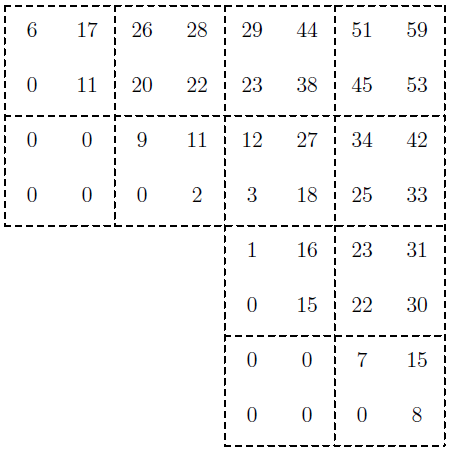
\includegraphics{fig2p2}
\end{center}
\caption{\small Explicit illustration of submatrices, just after quartering on the first iteration of {\it PATH0}}
\label{fig2p2}
\end{figure}

\begin{figure}[thb]
\begin{center}
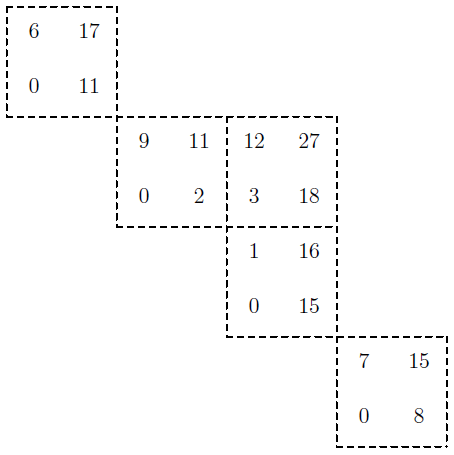
\includegraphics{fig2p3}
\end{center}
\caption{\small Explicit illustration of submatrices at the end of the first iteration {\it PATH0}}
\label{fig2p3}
\end{figure}

We illustrate {\it PATH0} using path $P$ as in Fig. \ref{fig2p2}, with $k=3$.
First we set $\lambda_1$ to 0 and $\lambda_2$ to $\infty$.
We initialize the set $\cal M$ to the set consisting of
the four $4 \times 4$ submatrices of the matrix $M(P)$.
On the first iteration of the while-loop,
$R= \{59,3,28,0,31,0,0,0\}$ and $R'= \{59,3,28,31\}$.
The median of this set is $(28+31)/2 = 29.5$.
For $\lambda = 29.5$, no cuts are required, so we reset $\lambda_2$ to 29.5.
Then we recompute $R'$ to be $\{3,28\}$, whose median is $(3+28)/2 = 15.5$. 
For $\lambda = 15.5$, 1 cut is required, so we reset $\lambda_2$ to 15.5. 
We discard the submatrix with all values less than or equal to $\lambda_1$, leaving three submatrices. 
We quarter these submatrices into 12 submatrices as shown in Fig. \ref{fig2p2}.
Of these 12 submatrices, five have all values too large, and two have all values too small.
We discard them, leaving the five submatrices pictured in Fig. \ref{fig2p3}.

On iteration 2, $R= \{17,0,27,3,11,0,16,0,15,0\}$, and $R'= \{3,11,15\}$.
The median of this set is $11$.
For $\lambda = 11$, 3 cuts are required, so we reset $\lambda_1$ to 11.
Then we recompute $R'$ to be $\{15\}$, whose median is $15$.
For $\lambda = 15$, 2 cuts are required, so we reset $\lambda_2$ to 15.
There are no submatrices with all values at least 15.5, and one submatrix with all values at most 11, and we discard the latter.
We quarter the remaining four submatrices, giving 16 submatrices of dimension $1 \times 1$, of which all but the one containing $12$ are either too large or too small.
On iteration 3, $R=\{12\}$, $R'=\{12\}$, and the median is $12$.
For $\lambda = 12$, 3 cuts are required, so we reset $\lambda_1$ to 12.
At this point, all values are discarded, so that the revised $R'$ is empty, and a second selection is not performed on iteration 3.
All submatrices will be discarded from $\cal M$, and {\it PATH0} will terminate with $\lambda_1 = 12$ and $\lambda_2 = 15$, and output $\lambda^*=12$.
\bigskip

\begin{theorem}
\label{thm:2:2}
Algorithm {\it PATH0} finds a max-min partition of a path of $n$
weighted vertices in $O(n \log n)$ time.
\end{theorem}
\begin{proof}
Correctness follows from the correctness of {\it FTEST0}, from the fact that all possible candidates for $\lambda^*$ are included in $M(P)$, and from the fact that each value discarded is either at most $\lambda_1$ or at least $\lambda_2$.

By Lemma \ref{lem:2:1}, {\it PATH0} will take $O(n)$ total time, exclusive of the feasibility tests, and will produce a sequence of $O( \log n )$ values to be tested.
It follows that the total time for all feasibility tests is $O(n \log n)$.
\end{proof}

The time for {\it PATH0} corresponds to the times achieved by Megiddo and Cole
for the path problem.
We show how to do better in Section \ref{sec:path}.

We next describe a simple approach {\it TREE0} to the max-min problem on a tree.
We first define an {\it edge-path-partition} of a tree
rooted at a vertex of degree 1.
Partition the edges of the tree into paths,
where a vertex is an endpoint of a path
if and only if it is of degree not equal to 2 with respect to the tree.
Call any path in an edge-path-partition
that contains a leaf in the tree a {\it leaf-path}.
As an example, consider the vertex-weighted tree in Fig. \ref{tfig2p3}(a).
Fig. \ref{tfig2p3}(b) shows the edge-path-partition for $T$.
There are 7 paths in the partition, as shown.
Four of these paths are leaf-paths.

\begin{figure}[thb]
\begin{center}
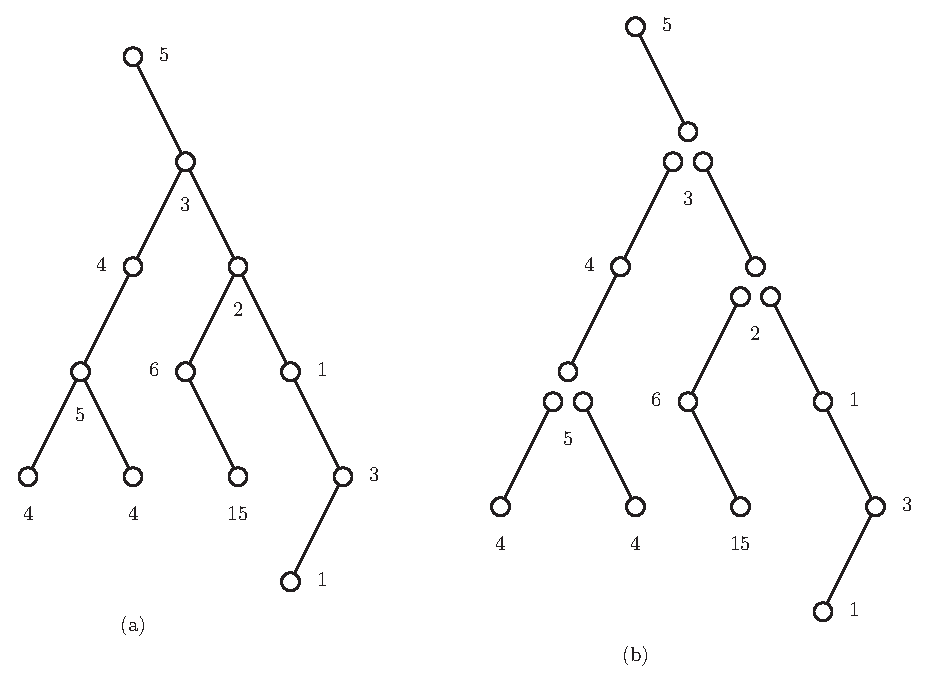
\includegraphics[scale=0.9]{tfig2p3}
%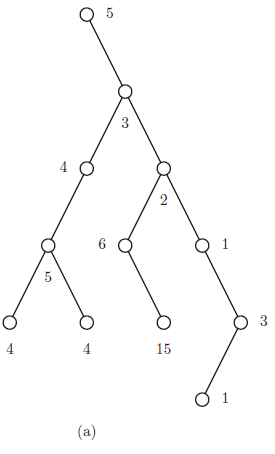
\includegraphics{tfig2p3a}
%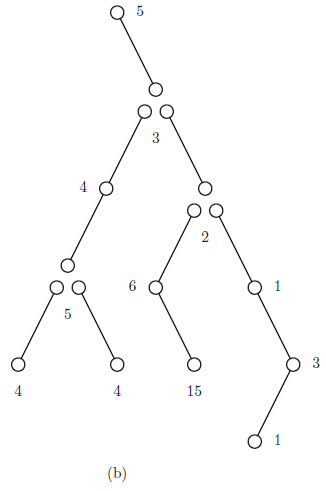
\includegraphics{tfig2p3b}
\end{center}
\caption{\small An edge-path-partition for $T$}
\label{tfig2p3}
\end{figure}

\begin{figure}[thb]
\begin{center}
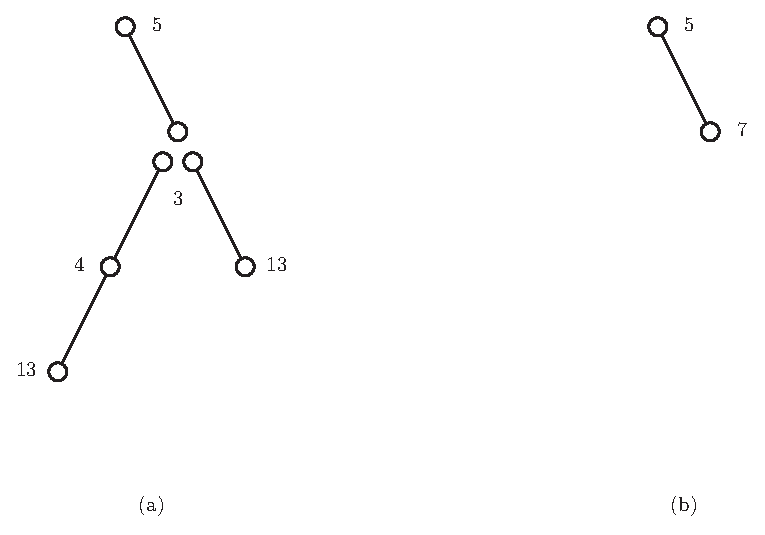
\includegraphics{tfig2p4}
\end{center}
\caption{\small The edge-path-partition of the resulting tree after all leaf-paths are deleted}
\label{tfig2p4}
\end{figure}

We now proceed with the approach for the tree.
Below are the three routines 
{\it TREE0\_init\_mat},
{\it TREE0\_test\_val},
and {\it TREE0\_update\_mat}.
The basic idea is to perform the search first on the leaf-paths,
and thus determine which edges in the leaf-paths should be cut.
When no search value on a leaf-path is contained in the open interval
$(\lambda_1, \lambda_2)$,
we prune the tree and repeat the process. 
We use the straightforward feasibility test described earlier.

The determination of cuts and pruning of the tree proceeds as follows.
If $T$ contains more than one leaf, do the following.
For each leaf-path $P_j$,
infer the cuts in $P_j$ such that each component in turn going up in $P_j$,
except the highest component on $P_j$, has total weight
as small as possible but greater than $\lambda_1$.
Delete all vertices beneath the top vertex of each leaf-path $P_j$,
and add to the weight of the top vertex in $P_j$
the weight of the other vertices in the highest component of $P_j$.
This leaves a smaller tree in which all leaf-paths
in the original tree have been deleted.
The smaller tree has at most half of the number of leaves of $T$.
Reset $T$ to be the smaller tree, and $k$ to be
the number of cuts remaining to be made in this tree.

\bigskip
\sspace
\noindent
{\it TREE0\_init\_mat}:\vspace{.05in}\\
$\T $ Initialize $T$ to be the tree rooted at a vertex of degree 1.\\
$\T $ Concatenate the leaf-paths of $T$ together, yielding path $P'$.\\
$\T $ Split sorted matrix $M(P')$ for the path $P'$ into 4 square submatrices. \\
$\T $ Let $\cal M$ be the set containing these four square submatrices.

\bigskip
\noindent
{\it TREE0\_test\_val}:\vspace{.05in}\\
$\T $ (Identical to {\it PATH0\_ident\_val}, \\
$\T \T$ except that {\it FTEST0} is called with argument $T$ rather than $P$).

\bigskip
\noindent
{\it TREE0\_update\_mat}:\vspace{.05in}\\
$\T$ Call {\it PATH0\_update\_mat} on $\mathcal{M}$.\\
$\T$ $\IF$ ${\cal M}$ is empty and $T$ is not a path \\
$\T$ $\TN$ \\
$\T \T$ $\FO$ each leaf-path of $T$ $\DO$ \\
$\T \T \T$ Determine cuts on the leaf-path, and decrease $k$ accordingly.\\
$\T \T \T$ Add to the weight of the top vertex the total weight of the\\
$\T \T \T \T$ other vertices in the highest component of the leaf-path.\\
$\T \T \T$ Delete from $T$ all vertices in the leaf-path except the top vertex.\\
$\T \T$ $\EF$ \\
$\T \T$ Concatenate the leaf-paths of $T$ together, yielding new path $P'$.\\
$\T \T$ Split sorted matrix $M(P')$ for path $P'$ into 4 square submatrices. \\
$\T \T$ Let $\cal M$ be the set containing these four square submatrices.\\
$\T$ $\EI$ 
 
\dspace
\bigskip


As an example we consider the max-min problem on the tree shown
in Fig. \ref{tfig2p3}(a), with $k=3$.
In the initialization,
four leaf-paths are identified and concatenated together,
giving the path $P' = 4, 5, 4, 5, 15, 6, 2, 1, 1, 3, 2$.
Once all search values associated with $P'$ are resolved,
$\lambda_1 = 10$ and $\lambda_2 = 13$. 
We place one cut between the vertices of weight 15 and 6, and reset $k$ to 2.
We add the weights of the two leaves of weight 4 to the weight of their parent, giving it weight 13.
We add the weights of all descendants of the vertex with weight 2, except the weight of 15, to the vertex of weight 2, giving it a weight also of 13.
Then we delete all edges in the leaf-paths. 
Fig. \ref{tfig2p4}(a) shows the edge-path-partition of the resulting tree.
There are two leaf-paths in this partition, with vertex weights 13, 4, and 3 on one, and 13 and 3 on the other.
We form the path $P' = 13, 4, 3, 13, 3$. 
Once we have resolved all search values associated with $P'$, we still have $\lambda_1 = 10$ and $\lambda_2 = 13$.
We can then place two cuts, above each of the vertices of weight 13,
and reset $k$ to 0. 
We add the weight of the vertex of weight 4 to its parent, giving it weight 7.
Then we delete all edges in the leaf-paths.
The edge-path-partition of the resulting tree is shown in Fig. \ref{tfig2p4}(b).
There is just one leaf-path in this partition,
with vertex weights 5 and 7.
Once all search values associated with $P'$ are resolved,
we have $\lambda_1 = 12$ and $\lambda_2 = 13$.
Since the tree consists of a single path, the algorithm then terminates with $\lambda^*=12$.
\bigskip

\begin{theorem}
\label{thm:2:3}
Algorithm {\it TREE0} finds a max-min partition of a tree of $n$
weighted vertices in $O(n (\log n)^2)$ time.
\end{theorem}
\begin{proof}
For correctness of the tree algorithm,
note that $\lambda_1$ always corresponds to a feasible value,
that all possible values resulting from leaf paths
are represented in $M(P')$,
and that the cuts are inferred on leaf-paths assuming (correctly)
that any subsequent value $\lambda$ to be tested
will have $\lambda > \lambda_1$.

We analyze the time as follows.
By Lemma \ref{lem:2:1}, resolving the path $P'$ will
use $O(\log n)$ feasibility tests,
and time exclusive of feasibility tests of $O(n)$.
Since each feasibility test takes $O(n)$ time,
the feasibility tests will use $O(n \log n)$ time.
Since resolving the path $P'$ will at least halve the number of leaves
in the tree, the number of such paths until the final version of $P'$ is $O(\log n)$.
Thus the total time to partition the tree by this method
is $O(n (\log n)^2)$.
\end{proof}

The time for {\it TREE0}
beats the time of $O(n(\log n)^3)$ for Megiddo's algorithm,
and matches the time of $O(n(\log n)^2)$ for Cole's algorithm.
We show how to do better for the max-min problem in Section \ref{sec:tree}.
\bigskip

